\documentclass[10pt,aspectratio=169,mathserif]{beamer}
\usepackage{nju}			 %导入 nju 模板宏包
\usepackage[UTF8]{ctex}      %导入 ctex 宏包,添加中文支持
\usepackage{xeCJK}
\usepackage{amsmath,amsfonts,amssymb,bm}   %导入数学公式所需宏包
\usepackage{color}			 %字体颜色支持
\usepackage{graphicx,hyperref,url}
\usepackage{listings}
\usepackage{booktabs}
\usepackage{multirow}

\beamertemplateballitem		%设置 Beamer 主题
\catcode`\。=\active        %或者=13
\newcommand{。}{.}         %将正文中的“。”号转换为“.”。

\AtBeginSection[]
{
  \begin{frame}
    \frametitle{提纲}
    \tableofcontents[currentsection]
  \end{frame}
}



\title{论文题目}	        %首页信息设置

\author[毛女神]{            %个人信息设置
    毛女神\\[0.3cm]
    15XXXXXXXX\\[0.3cm]
    匡亚明学院}

\date{\today}



\begin{document}

\begin{frame}
\titlepage
\end{frame}

\begin{frame}
\frametitle{提纲}
\tableofcontents
\end{frame}


\section{第一章标题}

\begin{frame}{标题}
内容内容内容内容内容内容内容内容内容内容内容内容内容内容内容内容内容内容内容
\end{frame}

\begin{frame}{列表}
\begin{itemize}
    \item 内容内容内容内容内容内容内容内容内容内容
    \begin{itemize}
        \item level 2
        \item xxx
    \end{itemize}
    \item 内容内容内容内容内容
\end{itemize}
\end{frame}

\begin{frame}{数字列表}
\begin{enumerate}
    \item 内容内容内容内容内容内容内容
    \item 内容内容内容内容
    \item 内容内容内容
\end{enumerate}
\end{frame}

\section{第二章标题}

\begin{frame}{图}
\begin{figure}
    \centering
    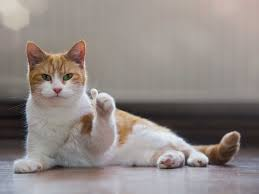
\includegraphics[width=8cm]{figure/1.jpg}
    \caption{猫}
\end{figure}
\end{frame}

\begin{frame}{公式}
\[
H=-\sum_{x\in U}{P(x) log⁡P(x)}
\]
\end{frame}

\begin{frame}{表}
\begin{table}
    \centering
    \caption{样表}
    \begin{tabular}{|p{2cm}|p{2cm}|p{2cm}|p{2cm}|p{2cm}|}
        \hline
        6608 & Raione & Yarerina & elone & Qoner \\ \hline
        Uanilon & Panilone & garine & 9808 & A108 \\ \hline
        Qanile & Janna & Daina & \$anione & Aanne \\ \hline
    \end{tabular}
\end{table}
\end{frame}

\begin{frame}{框图}
\begin{block}{信息熵}
    \[
    H=-\sum_{x\in U}{P(x) log⁡P(x)}
    \]
\end{block}
\end{frame}


\begin{frame}[c, plain]
  \begin{center}
    \Huge{\texttt{\textbf{Thank you!}}}\\[0.5cm]
    Q\&A
  \end{center}
\end{frame}


\end{document}
